\documentclass[12pt,a4paper]{article}

\usepackage[utf8]{inputenc}
\usepackage[T1]{fontenc}
\usepackage{babel}
\babelprovide[main,import]{english}
\usepackage[a4paper,margin=2.5cm]{geometry}
\usepackage{lmodern}
\usepackage{microtype}
\usepackage{amsmath}
\usepackage{booktabs}
\usepackage{longtable}
\usepackage{array}
\usepackage{enumitem}
\usepackage{tabularx}
\usepackage{graphicx}
\usepackage{tikz}
\usetikzlibrary{positioning}
\usepackage{eso-pic}
\usepackage{listings}
\usepackage{xcolor}
\usepackage{hyperref}
\usepackage{fancyhdr}
\usepackage{lastpage}

\definecolor{blueuh}{HTML}{123B63}
\definecolor{lightblue}{HTML}{EAF2F8}
\definecolor{orangeuh}{HTML}{B86B1B}
\lstset{basicstyle=\ttfamily\scriptsize,breaklines=true,breakatwhitespace=false,columns=fullflexible,frame=single,keepspaces=true,showstringspaces=false,literate={á}{{\'a}}1 {Á}{{\'A}}1 {í}{{\'i}}1 {Í}{{\'I}}1 {ó}{{\'o}}1 {Ó}{{\'O}}1 {️}{}1 {📄}{[PDF]}5 {🖼}{[IMG]}5}
\hypersetup{colorlinks=true,linkcolor=blueuh,urlcolor=blueuh,pdftitle={Database Design - Delivery Routes},pdfauthor={Digimons Team}}
\setlength{\parindent}{0pt}
\setlength{\parskip}{6pt}
\renewcommand{\arraystretch}{1.2}
\setlist[itemize]{leftmargin=*,itemsep=2pt}
\setlist[enumerate]{leftmargin=*,itemsep=4pt}
\pagestyle{fancy}
\setlength{\headheight}{15pt}
\fancyhf{}
\lhead{Databases II}
\rhead{Database Design}
\cfoot{\thepage\ of \pageref{LastPage}}
\renewcommand{\headrulewidth}{0.4pt}
\newcommand{\field}[1]{\texttt{#1}}
\AddToShipoutPictureBG{%
	\begin{tikzpicture}[remember picture,overlay]
		\node[opacity=0.08] at (current page.center) {
\includegraphics[width=0.72\paperwidth]{../MATCOM.png}};
	\end{tikzpicture}%
}

\begin{document}

\begin{titlepage}
\thispagestyle{empty}
\begin{center}
\vspace*{1cm}
{\Large \textbf{UNIVERSITY OF HAVANA}}\\[0.35cm]
{\large Faculty of Mathematics and Computer Science}\\[1.6cm]
{\Large \textbf{DATABASES II}}\\[1.5cm]
{\rule{\textwidth}{1pt}}\\[0.5cm]
{\huge \textbf{Report: Database Design}}\\[0.45cm]
{\Large Management for the Automatic Generation of Delivery Routes}\\[0.5cm]
{\rule{\textwidth}{1pt}}\\[1.5cm]
\begin{tabular}{ll}
\textbf{Academic year:} & 2026--2027 \\
\textbf{Team:} & Digimons
\end{tabular}
\vfill
\small
\begin{tabular}{>{\raggedright\arraybackslash}p{6.6cm}c p{3.1cm} p{3.7cm}}
\toprule
\textbf{Member} & \textbf{Group} & \textbf{Telegram} & \textbf{GitHub}\\
\midrule
Karla Díaz Saura & C312 & @kdiazsr & Krli01\\
Manuel Enrique Cardoso Martínez & C312 & @ManuEC04 & ManuEC04\\
Leonardo Peláez Ascención & C312 & @leosoyyoxd & Brand-Leo\\
Jorge Luis Herrera Cecilia & C312 & @Jorge\_Lhc & Jorge-Luis-Herrera\\
José Alejandro Albanés Febles & C311 & @cuban\_developer & JoseAlejandro0508\\
\bottomrule
\end{tabular}
\vfill
\textit{Report prepared according to the Methodological Guidelines for Databases II.}
\end{center}
\end{titlepage}

\tableofcontents
\newpage

\section{Project title}
\textbf{Management for the Automatic Generation of Delivery Routes.}

\section{Analysis and reformulation of requirements}

\subsection{General description}
The project starts from a practical need: to bring order to a delivery operation involving orders, centers, zones, coordinators, supervisors, and drivers. The web application will register orders and stops, organize territorial coverage, generate routes, validate plans, execute deliveries, and analyze their results. The database will follow that entire process so that every decision can be traced from order entry through delivery or rescheduling.

The solution combines a relational model for transactional information with an external graph engine for the dynamic network of roads and transit points. This separation enables efficient queries and alternative-route traversal without introducing into the relational schema a structure that changes and is traversed continuously.

\subsection{Actors and responsibilities}
\begin{longtable}{p{0.32\textwidth}p{0.62\textwidth}}
\toprule
\textbf{Actor} & \textbf{Main responsibilities}\\
\midrule
Administrator & Manage users and general parameters; prevent duplicate orders and incompatible route assignments.\\
Logistics coordinator & Register and classify orders, operate in authorized centers, select loads, generate routes, and resolve assigned rescheduling requests.\\
Operations supervisor & Review routes, approve or reject them, request modifications, and record observations.\\
Driver & Consult assigned routes, execute stops, register deliveries and incidents, and request rescheduling.\\
\bottomrule
\end{longtable}

\subsection{Reformulated functional requirements}
\begin{enumerate}
\item \textbf{Authentication and authorization.} The system will centralize user identity and apply permissions according to four roles: administrator, logistics coordinator, operations supervisor, and driver. The hierarchy is total and disjoint: every operational user belongs to one subtype and does not simultaneously belong to incompatible subtypes.
\item \textbf{Centers, zones, and stops.} Distribution centers, their covered zones, and destination stops will be registered. A center may cover several zones, and a zone may be served by several centers.
\item \textbf{Order registration.} An authorized coordinator will enter each order, specifying its description, delivery type (parcel, document, or perishable), priority (low, medium, or urgent), origin center, and destination stop.
\item \textbf{Automatic route generation.} The system will select orders and generate a route considering vehicle capacity, territorial distribution, delivery types, priority, and balancing criteria. The parameters used will be stored with the route.
\item \textbf{Supervision.} Every proposed route may be reviewed by a supervisor. The review result, date, and observations will be preserved for auditing.
\item \textbf{Assignment and execution.} An approved route may be assigned to a driver authorized for the corresponding center. The system will prevent the driver from having two incompatible active routes.
\item \textbf{Deliveries and rescheduling.} The driver will record the result of each delivery and its observations. In case of failure, the driver may create a rescheduling request and designate the coordinator who will resolve it; the manual result will be preserved.
\item \textbf{Reports and export.} All users may consult tabular and graphical results, sort columns, and export information to PDF.
\end{enumerate}

\subsection{Informational requirements}
The database must support at least the following queries:
\begin{enumerate}
\item Routes generated for a center, including creator, creation date, and parameters.
\item Most frequently managed orders in final routes, classified by priority and zone.
\item Routes validated by a supervisor, including date and observations.
\item Driver performance on a route, grouped by priority and on-time delivery rate.
\item Comparison of routes from several centers by zone, priority, and criteria compliance.
\item Correlation between priority and performance by center; identification of the ten orders with the highest non-compliance rate, their coordinator and center; and comparison between drivers who requested rescheduling and the average on-time rate of their fleets.
\end{enumerate}

\subsection{Non-functional requirements}
\begin{itemize}
\item \textbf{Performance and concurrency:} frequent queries about availability and deliveries must respond with low latency even when several coordinators are connected.
\item \textbf{Availability:} driver and in-progress stop status must be reflected promptly during the workday.
\item \textbf{Scalability and maintainability:} the architecture must be decoupled, documented, modular, and prepared for new functionality.
\item \textbf{Cross-platform operation:} the web application must run in the environments expected by the team and users.
\item \textbf{Development quality:} the project requires version control, planning, documented code, at least two design patterns, and unit tests for both backend and frontend.
\item \textbf{Territorial network:} the connection network will be managed independently through a graph structure appropriate for dynamic traversal and searches.
\end{itemize}

\section{Proposed technology stack and architecture}

\subsection{Technology stack}
The solution will be implemented as a cross-platform web application organized into decoupled services. The selected technologies address the need for a maintainable interface, a strictly validated API, a transactional relational model, and a specialized component for the dynamic road network.

\begin{longtable}{p{0.25\textwidth}p{0.28\textwidth}p{0.39\textwidth}}
\toprule
\textbf{Layer} & \textbf{Technologies} & \textbf{Responsibility}\\
\midrule
Presentation & React, TypeScript, Vite, React Router & Web interface, navigation, forms, route queries, and report visualization.\\
State and data & TanStack Query & API consumption, caching, synchronization, and loading or error states.\\
Visualization & Recharts & Charts for priorities, compliance, performance, and center comparison.\\
Backend & Python, FastAPI, Pydantic & REST API, data validation, authentication, and use-case coordination.\\
Relational persistence & PostgreSQL, SQLAlchemy, Alembic & Users, orders, centers, routes, deliveries, rescheduling, and integrity constraints.\\
Graph persistence & Neo4j & Zones, roads, transit points, distances, estimated times, and alternative routes.\\
Testing & Pytest, Vitest, React Testing Library & Backend and frontend unit tests, including critical business rules.\\
Execution & Docker Compose & Reproducible environment for frontend, backend, PostgreSQL, and Neo4j.\\
Collaboration & GitHub, GitHub Projects, GitHub Actions & Version control, planning, review, and automated test execution.\\
\bottomrule
\end{longtable}

\subsection{Architecture and communication}
The architecture will follow a layered approach. React will communicate with FastAPI through a REST API over HTTPS. FastAPI will separate HTTP routes, application services, repositories, and integrations with PostgreSQL and Neo4j. PostgreSQL will be the source of truth for transactional operations; Neo4j will be used to traverse the territorial network and suggest alternative routes. Communication between both stores will be coordinated by the service layer and not by the user interface.

\begin{itemize}
\item \textbf{Presentation layer:} typed React components with TypeScript, validated forms, and operational and reporting views.
\item \textbf{API layer:} versioned REST endpoints, Pydantic schemas, and consistent error handling.
\item \textbf{Application layer:} use cases for registering orders, generating routes, validating routes, recording deliveries, and resolving rescheduling requests.
\item \textbf{Persistence layer:} separate repositories for PostgreSQL and Neo4j, with relational transactions and specialized graph queries.
\item \textbf{Security layer:} access and refresh tokens, Argon2-protected passwords, and authorization by role and enabled center.
\end{itemize}

\subsection{Patterns, quality, and operation}
The project will apply the \textbf{Repository} pattern to isolate data access, \textbf{Service Layer} to centralize business rules, and \textbf{Strategy} to support new balancing criteria without modifying the general route-generation flow. Code will be organized by responsibility, with descriptive names, documentation for public functions, and validation at each service boundary.

Unit tests will cover at least role authorization, duplicate-order prevention, exclusive driver assignment, criteria-based generation, delivery recording, and rescheduling creation. The frontend will be tested with Vitest and React Testing Library; the backend will be tested with Pytest. GitHub Actions will run these tests automatically on relevant changes.

Configuration will be managed through environment variables and an example file. Docker Compose will provide a reproducible local environment. The repository must include dependency manifests, a `.gitignore` file, the services required for local execution, and visible planning in GitHub Projects with tasks, assignees, statuses, dates, and milestones.

\section{Extended Relational Conceptual Model (ERCM)}

\subsection{Conceptual view}
The ERCM is organized around the root entity \textbf{USER} and a total, disjoint ISA specialization into LOGISTICS\_COORDINATOR, DRIVER, OPERATIONS\_SUPERVISOR, and ADMINISTRATOR. Territorial and operational entities are connected through relationships with explicit cardinalities. Attributes belonging to M:N relationships are represented by \textbf{ROUTE\_STOP} and \textbf{ROUTE\_CRITERION} in the relational schema.

\begin{figure}[htbp]
\centering
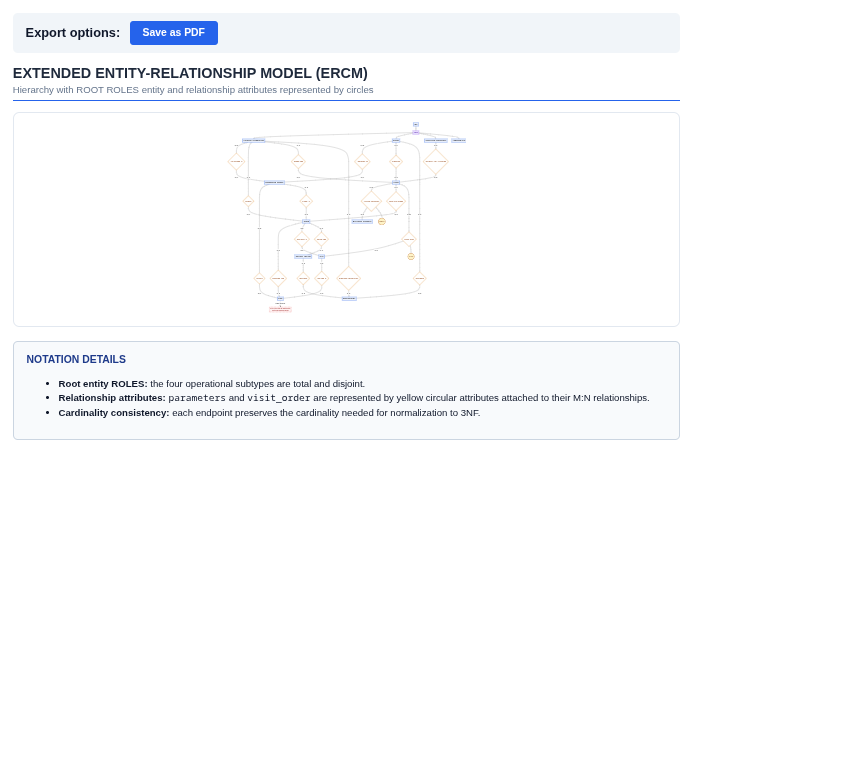
\includegraphics[width=\textwidth,height=0.58\textheight,keepaspectratio]{../MERX_english.pdf}
\caption{Extended Entity-Relationship Model (ERCM).}
\label{fig:ercm}
\end{figure}

\subsection{Main entities and relationships}
\begin{itemize}
\item \textbf{Users and roles:} USER centralizes name, email, credentials, status, and session renewal. Each subtype adds its specific attributes.
\item \textbf{Territory:} DISTRIBUTION\_CENTER is related to ZONE through COVERS; a STOP is located in a zone. Road topology remains outside the relational model.
\item \textbf{Load:} ORDER is entered by a coordinator, stored at a center, and delivered to a stop. A route contains the selected orders, resolving the connection trap between planning and execution.
\item \textbf{Planning:} ROUTE is generated by a coordinator, originates at a center, may be validated by a supervisor, and is executed by a driver. ROUTE\_STOP stores visit order and ROUTE\_CRITERION stores the applied parameters.
\item \textbf{Traceability:} each DELIVERY\_RECORD documents an order; a failed delivery may originate a RESCHEDULING request submitted by a driver and resolved by a coordinator.
\end{itemize}

\section{Integrity constraints}

\subsection{Entity integrity}
Every table has a non-null and unique primary key. Primary keys include `id\_user`, `id\_coordinator`, `id\_driver`, `id\_supervisor`, `id\_admin`, `id\_center`, `id\_zone`, `id\_stop`, `id\_order`, `id\_criterion`, `id\_route`, `id\_delivery`, and `id\_rescheduling`. Associative tables use composite keys such as `(id\_center,id\_zone)`, `(id\_route,id\_stop)`, and `(id\_route,id\_criterion)`.

\subsection{Referential integrity}
\begin{itemize}
\item Every user subtype references exactly one existing USER.
\item ORDER references an existing coordinator, center, and stop; the route is nullable until the order is dispatched.
\item STOP references an existing ZONE. CENTER\_ZONE relates only existing centers and zones.
\item ROUTE references the coordinator who generates it and its origin center; supervisor and driver may be null until those stages are completed.
\item ROUTE\_STOP and ROUTE\_CRITERION may reference only existing routes, stops, and criteria.
\item DELIVERY\_RECORD references an existing ORDER and RESCHEDULING references an existing delivery record.
\end{itemize}

\subsection{Business constraints}
\begin{enumerate}
\item \textbf{No duplicates:} a unique constraint will be defined over the attributes that identify the same business order, together with application-level validation.
\item \textbf{Authorization:} a coordinator may register orders or generate routes only for centers present in COORDINATOR\_CENTER.
\item \textbf{Exclusive assignment:} a driver may not have more than one incompatible active route; this will be guaranteed through transactional validation and a partial unique constraint where supported.
\item \textbf{Geographical consistency:} a stop must belong to a valid zone, and the center-zone combination must exist when orders or routes are assigned to a center.
\item \textbf{Criteria persistence:} parameters are stored as a snapshot in ROUTE\_CRITERION, so later changes to a criterion do not alter historical traceability.
\item \textbf{Valid rescheduling:} only a registered and unsuccessful delivery may generate a request; status and resolution date must be consistent.
\item \textbf{Controlled states:} priority, delivery type, order status, route status, and delivery result must be restricted to system-defined domains.
\end{enumerate}

\section{Assessment of design correctness}

\subsection{Functional dependencies and normalization}
From the attribute universe, the following representative functional dependencies are obtained:
\begin{align*}
\field{id\_user} &\rightarrow \text{general user data},\\
\field{id\_order} &\rightarrow \text{order data, coordinator, center, and stop},\\
\field{id\_stop} &\rightarrow \field{id\_zone},\\
\field{id\_route} &\rightarrow \text{dates, capacity, status, coordinator, and center},\\
(\field{id\_route},\field{id\_stop}) &\rightarrow \field{visit\_order},\\
(\field{id\_route},\field{id\_criterion}) &\rightarrow \field{configuration\_parameters}.
\end{align*}
The dependency $\field{id\_order} \rightarrow \field{id\_zone}$ is not kept as an independent dependency because it follows transitively from $\field{id\_order} \rightarrow \field{id\_stop}$ and $\field{id\_stop} \rightarrow \field{id\_zone}$. Removing this redundancy avoids update anomalies.

Synthesis by determinant produces, among others, USER, the role subtypes, DISTRIBUTION\_CENTER, ZONE, CENTER\_ZONE, STOP, ORDER, BALANCING\_CRITERION, ROUTE, ROUTE\_STOP, ROUTE\_CRITERION, COORDINATOR\_CENTER, DRIVER\_CENTER, DELIVERY\_RECORD, and RESCHEDULING. Each relation contains attributes that depend on its key, on the whole key, and on no non-key attribute; therefore, the resulting schema satisfies 3NF under the declared dependencies.

\subsection{Dependency preservation and lossless join}
Dependencies are preserved because every determinant and its dependent attributes appear in a synthesized relation. Foreign keys preserve the semantic links and allow the information to be reconstructed through lossless joins. The direct ROUTE--ORDER association prevents losing the relationship between an expedition and its load when a stop contains orders from different routes.

\subsection{Recommended implementation decisions}
\begin{itemize}
\item Use transactions to generate routes, assign drivers, and register deliveries.
\item Index foreign keys, operational statuses, dates, centers, and priorities to support reports.
\item Apply concurrency control when checking availability and confirming assignments.
\item Keep the road network in the graph engine and store in the relational model the references needed to connect stops and zones.
\item Implement a decoupled layered or modular architecture, apply at least two patterns, and provide unit tests for backend and frontend.
\end{itemize}

\section{Conclusions}
This design aims to make the database reflect the real operation rather than merely present a list of tables. Roles represent different responsibilities; orders retain their origin, destination, and status; routes keep the criteria used to generate them; and delivery records make it possible to understand what happened at each stop. Information therefore remains traceable when a route changes, a delivery fails, or a rescheduling request is created.

ISA specialization prevents common user data from being repeated, while associative relationships represent routes, stops, and applied criteria correctly. The road network is kept in a graph engine because its connections and traversals change more often than administrative data. This separation keeps the relational model understandable and leaves room to search for alternatives when a delivery cannot be completed as planned.

Keys, references, and business constraints protect data consistency, while 3NF normalization reduces duplication and update anomalies. The proposed technology stack also provides a realistic path from this model to a maintainable application, with an accessible interface, a validated API, automated tests, and a reproducible environment. The result does not attempt to settle every implementation detail, but it offers a solid, understandable, and verifiable foundation for building the system.

\section*{Sources used}
\addcontentsline{toc}{section}{Sources used}
\begin{itemize}
\item International Council on Systems Engineering. \textit{Requirements Engineering}, SEBoK v2.14. Available at: \url{https://www.sebokwiki.org/wiki/Requirements_Engineering}. Accessed October 9, 2026.
\item University of Cape Town. \textit{Chapter 6: Entity-Relationship Modelling}. Academic database material. Available at: \url{https://www.cs.uct.ac.za/mit_notes/database/htmls/chp06.html}. Accessed October 9, 2026.
\item University of Cape Town. \textit{Chapter 7: Enhanced Entity-Relationship Modelling}. Academic material on specialization, generalization, and ISA constraints. Available at: \url{https://www.cs.uct.ac.za/mit_notes/database/htmls/chp07.html}. Accessed October 9, 2026.
\item University of Cape Town. \textit{Chapter 8: Data Normalisation}. Academic material on functional dependencies and 1NF--3NF. Available at: \url{https://www.cs.uct.ac.za/mit_notes/database/htmls/chp08.html}. Accessed October 9, 2026.
\item PostgreSQL Global Development Group. \textit{Data Definition and Constraints}. Official documentation on keys, constraints, and referential integrity. Available at: \url{https://www.postgresql.org/docs/current/ddl-constraints.html}. Accessed October 9, 2026.
\item Neo4j, Inc. \textit{Get Started with Neo4j}. Official documentation on graph databases and Cypher. Available at: \url{https://neo4j.com/docs/getting-started/current/}. Accessed October 9, 2026.
\item React. \textit{React Documentation: Learn}. Official documentation on components and interface state. Available at: \url{https://react.dev/learn}. Accessed October 9, 2026.
\item FastAPI. \textit{FastAPI Documentation}. Official documentation on APIs, validation, and OpenAPI. Available at: \url{https://fastapi.tiangolo.com/}. Accessed October 9, 2026.
\item Docker. \textit{Get Started}. Official documentation on containers and reproducible environments. Available at: \url{https://docs.docker.com/get-started/}. Accessed October 9, 2026.
\item GitHub. \textit{About Projects}. Official documentation on planning with boards, milestones, and task tracking. Available at: \url{https://docs.github.com/en/issues/planning-and-tracking-with-projects/learning-about-projects/about-projects}. Accessed October 9, 2026.
\end{itemize}

\end{document}
